\chapter{Die natürlichen Zahlen}\label{ch:Kapitel01}
\section{Historische Betrachtung der natürlichen Zahlen}\label{sec:history}
Die \textit{natürlichen} Zahlen werden so genannt, da sie auf \enquote{natürliche Weise} beim Zählen verwendet werden. Auf dem Gebiet der heutigen Demokratischen Republik Kongo wurde im 20. Jahrhundert ein Knochen, der sogenannte \textit{Ishango-Knochen}, gefunden. Dieser Knochen wird auf die Zeit vor etwa 18'000 bis 20'000 Jahren vor unserer Zeitrechnung datiert. In dem Knochen sind ganz offensichtlich von Menschen einige Kerben eingeritzt worden. Die Bedeutung dieser Kerben ist nicht klar. Es wird jedoch angenommen, dass diese Kerben eine bestimmte Anzahl festhalten. 

Stellen wir uns vor, dass die Kerben die Anzahl der gefangenen Fische (\twemoji{tropical fish}) an einem bestimmten Tag darstellen. Gefangene Fische durch Kerben in einem Knochen zu repräsentieren, verlangt bereits einen recht hohen Grad an Abstraktion! Schliesslich haben gefangene Fische und Kerben in einem Knochen auf den ersten Blick keinen offensichtlichen Zusammenhang. Anstelle von Kerben in einem Knochen könnte die Fangmenge eines Tages auch durch die entsprechende Anzahl von Kieselsteinen oder durch (abstraktere) römische Numerale repräsentiert werden. Wichtig für uns ist, dass die konkrete Wahl der Darstellung, zumindest rein mathematisch betrachtet, unwichtig ist. Schliesslich stellen die verschiedenen Darstellungen alle dieselbe Anzahl von Fischen dar. Betrachten Sie \cref{tab:fische}. Mit dem Symbol \twemoji{tropical fish} meinen wir nicht ein Fisch-Emoji, sondern den eigentlich gefangenen Fisch. Die direkte Darstellung der Anzahl der gefangenen Fische durch sich selbst ist offensichtlich am wenigsten abstrakt. Die Darstellung durch Kerben oder Kieselsteine bedarf bereits einer nicht unerheblichen Abstraktion. Die Darstellungen durch das römische, dezimale und binäre Zahlensystem sind noch eine Stufe abstrakter.

\begin{table}[H]
    \centering
    \begin{tabular}{rrrrr}
    \textbf{Fische}  & \textbf{Kieselsteine}                                                                                          & \textbf{römisch}        & \textbf{binär} & \textbf{dezimal} \\ \hline
    (keine) & (keine)                                                                                               & nichts (nihil) & 0     & 0       \\
    $\twemoji{tropical fish}$ & \textbullet                                                                                         &     \romanNumeral{1}           & 1     & 1       \\
    $\twemoji{tropical fish}\twemoji{tropical fish}$        & \textbullet\textbullet                                                                              &      \romanNumeral{2}           & 10    & 2       \\
    $\twemoji{tropical fish}\twemoji{tropical fish}\twemoji{tropical fish}$        & \textbullet\textbullet\textbullet                                                                  &      \romanNumeral{3}           & 11    & 3       \\
    $\twemoji{tropical fish}\twemoji{tropical fish}\twemoji{tropical fish}\twemoji{tropical fish}$        & \textbullet\textbullet\textbullet\textbullet                                                       &       \romanNumeral{4}          & 100   & 4       \\
    $\twemoji{tropical fish}\twemoji{tropical fish}\twemoji{tropical fish}\twemoji{tropical fish}\twemoji{tropical fish}$        & \textbullet\textbullet\textbullet\textbullet\textbullet                                            &      \romanNumeral{5}           & 101   & 5       \\
    $\twemoji{tropical fish}\twemoji{tropical fish}\twemoji{tropical fish}\twemoji{tropical fish}\twemoji{tropical fish}\twemoji{tropical fish}$        & \textbullet\textbullet\textbullet\textbullet\textbullet\textbullet                                  &      \romanNumeral{6}           & 110   & 6       \\
    $\twemoji{tropical fish}\twemoji{tropical fish}\twemoji{tropical fish}\twemoji{tropical fish}\twemoji{tropical fish}\twemoji{tropical fish}\twemoji{tropical fish}$        & \textbullet\textbullet\textbullet\textbullet\textbullet\textbullet\textbullet                       &       \romanNumeral{7}          & 111   & 7       \\
    $\twemoji{tropical fish}\twemoji{tropical fish}\twemoji{tropical fish}\twemoji{tropical fish}\twemoji{tropical fish}\twemoji{tropical fish}\twemoji{tropical fish}\twemoji{tropical fish}$        & \textbullet\textbullet\textbullet\textbullet\textbullet\textbullet\textbullet\textbullet            &        \romanNumeral{8}         & 1000  & 8       \\
    $\twemoji{tropical fish}\twemoji{tropical fish}\twemoji{tropical fish}\twemoji{tropical fish}\twemoji{tropical fish}\twemoji{tropical fish}\twemoji{tropical fish}\twemoji{tropical fish}\twemoji{tropical fish}$        & \textbullet\textbullet\textbullet\textbullet\textbullet\textbullet\textbullet\textbullet\textbullet &       \romanNumeral{9}         & 1001  & 9      
    \end{tabular}
    \caption{mögliche Darstellungen der Anzahl gefangener Fische}
    \label{tab:fische}
\end{table}
\noindent
Die Zahl \textit{Null} hat eine lange und kontroverse Geschichte hinter sich. Vermutlich hatten die Römer kein explizites eigenes Symbol für die Null. Wir werden jedoch die Null als die erste (kleinste) natürliche Zahl auffassen.

\section{Unendlichkeit der natürlichen Zahlen und konstruktive Induktion}
Bereits aufgrund der kurzen Anekdote über die gefangenen Fische und Kieselsteine in \cref{sec:history} kann man sich denken, dass es unendlich viele natürliche Zahlen geben muss. Wieder denken wir uns eine natürliche Zahl als genau das Symbol, welches eine bestimme Anzahl an Kieselsteinen darstellt. Dann ist klar, dass es keine grösste natürliche Zahl geben kann, denn schliesslich kann stets ein weiterer Kieselstein hinzugefügt werden, was uns eine noch grössere Zahl liefert. Zu jeder natürlichen Zahl $n$, angefangen mit der $0$, erhalten wir (durch Hinzufügen eines Kieselsteins) eine weitere natürliche Zahl. Diese neue Zahl werden wir den \textit{Nachfolger} von $n$ nennen. Die folgenden Überlegungen dieses Kapitels formalisieren diese
Vorstellungen und stellen diese mathematisch präzise dar. Doch auch ohne mathematische Formeln können wir das folgende Gedankenexperiment durchführen. Angenommen Sie sind in der Lage Folgendes zu tun:
\begin{itemize}
    \item Sie können eine Treppe mit $0$ Stufen (ohne Stufen) bauen.
    \item Falls Sie bereits eine Treppe mit einer beliebigen (natürlichen) Anzahl von Stufen gebaut haben, dann können Sie diese Treppe um eine Stufe erweitern (siehe \cref{fig:treppe}).
\end{itemize}
Dann werden Sie es für glaubhaft halten, dass Sie eine Treppe mit beliebig vielen Stufen bauen können. Wie dieses Gedankenexperiment mit der mathematischen Definition der natürlichen Zahlen zusammenhängt, werden Sie im nächsten Abschnitt sehen.

\begin{figure}[H]
    \centering
\begin{subfigure}[b]{0.48\textwidth}
    \begin{tikzpicture}
    \newcommand{\stairs}{3}
    \newcommand{\width}{3.4}
    \newcommand{\riserheight}{0.6}
    \newcommand{\tread}{0.5}
    \begin{scope}[x={(1.2*\tread cm,-0.8*\tread cm)}, y={(1*\width cm,0.8*\width cm)}, z={(0 cm,\riserheight cm)}]
    \foreach \i in {1,...,\stairs} {
        \fill[DarkBlue!10] (\i-1,0,{\stairs-\i+1}) -- (\i-1,1,{\stairs-\i+1}) -- (\i,1,{\stairs-\i+1}) -- (\i,0,{\stairs-\i+1}) -- cycle;
        \fill[DarkBlue!40] (\i,0,{\stairs-\i}) -- (\i,1,{\stairs-\i}) -- (\i,1,{\stairs+1-\i}) -- (\i,0,{\stairs+1-\i}) -- cycle;
    }
    \draw[fill=DarkBlue!50] (0,0,0) -- (0,0,\stairs) \foreach \i in {1,...,\stairs} {-- (\i,0,{\stairs+1-\i}) -- (\i,0,{\stairs+1-\i-1})} -- cycle;
    \draw (0,0,\stairs) -- (0,1,\stairs)  \foreach \i in {1,...,\stairs} {-- (\i,1,{\stairs+1-\i}) -- (\i,1,{\stairs+1-\i-1})} -- (\stairs,0,0);
    \end{scope}
    \draw [-stealth](5.7,2) -- (6.7,2);
    \end{tikzpicture}
\end{subfigure}
\begin{subfigure}[b]{0.48\textwidth}
    \begin{tikzpicture}
    \newcommand{\STAIRS}{4}
    \newcommand{\width}{3.4}
    \newcommand{\riserheight}{0.6}
    \newcommand{\tread}{0.5}
    \begin{scope}[x={(1.2*\tread cm,-0.8*\tread cm)}, y={(1*\width cm,0.8*\width cm)}, z={(0 cm,\riserheight cm)}]
    \foreach \i in {1,...,\STAIRS} {
        \fill[DarkBlue!10] (\i-1,0,{\STAIRS-\i+1}) -- (\i-1,1,{\STAIRS-\i+1}) -- (\i,1,{\STAIRS-\i+1}) -- (\i,0,{\STAIRS-\i+1}) -- cycle;
        \fill[DarkBlue!40] (\i,0,{\STAIRS-\i}) -- (\i,1,{\STAIRS-\i}) -- (\i,1,{\STAIRS+1-\i}) -- (\i,0,{\STAIRS+1-\i}) -- cycle;
    }
    \draw[fill=DarkBlue!50] (0,0,0) -- (0,0,\STAIRS) \foreach \i in {1,...,\STAIRS} {-- (\i,0,{\STAIRS+1-\i}) -- (\i,0,{\STAIRS+1-\i-1})} -- cycle;
    \draw (0,0,\STAIRS) -- (0,1,\STAIRS)  \foreach \i in {1,...,\STAIRS} {-- (\i,1,{\STAIRS+1-\i}) -- (\i,1,{\STAIRS+1-\i-1})} -- (\STAIRS,0,0);
    \end{scope}
    \end{tikzpicture}
\end{subfigure}
\caption{Erweiterung einer Treppe um eine weitere Stufe.}
\label{fig:treppe}
\end{figure}

\section{Die Peano-Axiome}
Uns ist vollkommen bewusst, dass Sie bereits seit Ihrer Kindheit mit dem Konzept der natürlichen Zahlen vertraut sind. Sie konnten vermutlich schon als Kleinkind Gegenstände zählen und lernten spätestens in der Grundschule die Addition und Multiplikation natürlicher Zahlen kennen. Für diese einfachen Anwendungen reicht eine rein intuitive Beschreibung der natürlichen Zahlen vollkommen aus.

Sie werden jedoch festgestellt haben, dass mit fortschreitender schulischer Reife eine präzise Definition von Begriffen und Konzepten zunehmend an Bedeutung gewinnt. Auf der Stufe des Gymnasiums wird der bis dorthin rein intuitiv geprägte Begriff der natürlichen Zahlen durch das Konzept der \textit{Mengen} formalisiert. Ab dann wird von der \textit{Menge der natürlichen Zahlen}, bezeichnet durch das Symbol $\N$, gesprochen.

\section{Informale Definition der natürlichen Zahlen}
In Lehrbüchern des Gymnasiums (siehe zum Beispiel \cite{ArminBarth}\footnote{Dieses Buch bietet allerdings auch eine alternative Definition der natürlichen Zahlen an.}) wird die Menge der natürlichen Zahlen typischerweise wie folgt definiert:
\begin{definition}[Informale Definition der natürlichen Zahlen]{definition:Ninformal}
Die Menge
\begin{align*}
    \N := \lrc{0,1,2,3,4,\ldots}
\end{align*}
wird als die Menge der \textbf{natürlichen Zahlen} bezeichnet.
\end{definition}
Man beginnt also bei $0$ und zählt dann unbegrenzt weit nach vorne. In einem gewissen Sinne beantwortet \cref{definition:Ninformal} die Frage, was natürliche Zahlen sind: Eine natürliche Zahl ist ein Element der Menge $\N$. Dennoch ist die Definition nicht sehr befriedigend, denn sie beantwortet nicht die Frage, was $\N$ selbst ist. \cite{TerenceTao} Wir werden nicht von dieser Definition Gebrauch machen, sondern eine nützlichere Definition entwickeln. 

Der folgende Abschnitt ist teilweise inspiriert durch die entsprechenden Teile in den hervorragenden Büchern \cite{TerenceTao} und \cite{AmannEscher1}.

Bei näherer Betrachtung wirft die informale \cref{definition:Ninformal} insbesondere die folgenden drei Fragen auf:
\begin{enumerate}
    \item Woher wissen wir, dass wir beliebig lange weiter vorwärts zählen können, ohne schliesslich (wie bei einer Uhr) wieder bei der $0$ anzukommen?
    \item Wie sollen nun Operationen wie die Addition, Multiplikation und die Potenz definiert werden?
\end{enumerate}
Die zweite Frage wollen wir zuerst besprechen. Komplizierte Operationen können durch einfachere Operationen ausgedrückt werden. So ist Potenzieren lediglich wiederholtes Multiplizieren und Multiplizieren wiederum wiederholtes Addieren. Zum Beispiel sind $5^3$ nichts weiter als drei Fünfer miteinander multipliziert und $6\cdot 3$ lediglich sechs Dreien miteinander addiert. Wie sieht es mit der Addition aus? Die Addition kann durch wiederholtes \textit{Inkrementieren} oder \textit{Vorwärtszählen} realisiert werden. Bei der Addition $4+3$ wird die Vier dreimal inkrementiert (wir zählen von der Vier aus dreimal vorwärts). Inkrementieren scheint eine fundamentale Operation zu sein, welche sich nicht auf eine noch einfachere Operation reduzieren lässt.

Eine sinnvolle Definition der natürlichen Zahlen scheint also das Inkrementieren als fundamentales Konzept zu verwenden. Für eine natürliche Zahl $n$ werden wir im Folgenden mit $\nu(n)$ das Inkrement von $n$ bezeichnen. Wir werden $\nu(n)$ auch den \tib{Nachfolger}\index{Nachfolger} von $n$ nennen. Zum Beispiel gilt $3=\nu(2), 4 = \nu(3) = \nu(\nu(2))$ und so weiter. Das Inkrementieren liefert uns also einen \enquote{Zählvorgang}, der bei 0 beginnt. Die bisherigen Überlegungen lassen vermuten, dass wir $\N$ als die Menge mit den Elementen
\begin{align*}
    0, \nu(0), \nu(\nu(0)), \nu(\nu(\nu(0))), \nu(\nu(\nu(\nu(0)))), \nu(\nu(\nu(\nu(\nu(0))))), \ldots
\end{align*}
ansehen wollen. Diese Menge enthält $0$ und alle Objekte, welche aus $0$ durch Inkrementieren erhalten werden können. Sie wissen bereits, dass fundamentale (nicht beweisbare) Annahmen in der Mathematik als \textit{Axiome} bezeichnet werden. Bislang haben wir zwei fundamentale Annahmen bezüglich der Menge $\N$ der natürlichen Zahlen getroffen. Diese fassen wir in zwei Axiomen zusammen:
\axiom{axiom:a1}
{Die $0$ liegt in $\N$.}
\axiom{axiom:a2}
{Falls $n$ in $\N$ liegt, dann liegt auch der Nachfolger $\nu(n)$ von $n$ in der Menge $\N$.}

\noindent
Dies sind die ersten zwei von insgesamt fünf Axiomen, welche zusammen bekannt sind als die \tib{Peano-Axiome}\index{Peano-Axiome} der natürlichen Zahlen. Die Peano-Axiome sind benannt nach dem italienischen Mathematiker \textit{Giuseppe Peano}, welcher diese Axiome im Jahr 1889 formulierte.

\bemerkungen{-}{}
{Beachten Sie, dass \cref{axiom:a2} lediglich aussagt, dass der Nachfolger $\nu(n)$ einer natürlichen Zahl $n$ wieder eine natürliche Zahl ist. Das Axiom sagt nichts darüber aus, wie dieser Nachfolger lautet.}
{Manche Autorinnen und Autoren ziehen es vor, den \enquote{Zählvorgang} nicht bei $0$, sondern bei $1$ zu beginnen. Dies ist mathematisch ohne Bedeutung. \cite{AmannEscher1}}
{Wir definieren $1:=\nu(0)$, $2:=\nu(1)=\nu(\nu(0))$, $3:=\nu(2)=\nu(\nu(\nu(0)))$ und so weiter. Anstelle von
\begin{align*}
    0, \nu(0), \nu(\nu(0)), \nu(\nu(\nu(0))), \nu(\nu(\nu(\nu(0)))), \nu(\nu(\nu(\nu(\nu(0))))), \ldots
\end{align*}
schreiben wir üblicherweise $0, 1, 2, 3, 4, 5, \ldots$
}
In \cref{sec:history} haben wir bereits begründet, warum die konkrete Darstellung einer Zahl nicht von Bedeutung ist. Wir haben \cref{tab:fische} um eine Spalte erweitert:
\begin{table}[H]
    \centering
    \begin{tabular}{rrrrrr}
    \textbf{Fische}  & \textbf{Kieselsteine} & \textbf{römisch} & \textbf{binär} & \textbf{dezimal}  & \textbf{Nachfolger} \\ \hline
    (keine) & (keine) & nichts (nihil) & 0     & 0     & {\tiny 0}  \\
    $\twemoji{tropical fish}$ & \textbullet                                                                                         &     \romanNumeral{1}           & 1     & 1    & {\tiny $\nu(0)$}   \\
    $\twemoji{tropical fish}\twemoji{tropical fish}$        & \textbullet\textbullet                                                                             &      \romanNumeral{2}           & 10    & 2  & {\tiny $\nu(\nu(0))$}     \\
    $\twemoji{tropical fish}\twemoji{tropical fish}\twemoji{tropical fish}$        & \textbullet\textbullet\textbullet                                                                   &      \romanNumeral{3}           & 11    & 3   & {\tiny $\nu(\nu(\nu(0)))$}     \\
    $\twemoji{tropical fish}\twemoji{tropical fish}\twemoji{tropical fish}\twemoji{tropical fish}$        & \textbullet\textbullet\textbullet\textbullet                                                        &       \romanNumeral{4}          & 100   & 4  & {\tiny $\nu(\nu(\nu(\nu(0))))$}     \\
    $\twemoji{tropical fish}\twemoji{tropical fish}\twemoji{tropical fish}\twemoji{tropical fish}\twemoji{tropical fish}$        & \textbullet\textbullet\textbullet\textbullet\textbullet                                            &      \romanNumeral{5}           & 101   & 5   & {\tiny $\nu(\nu(\nu(\nu(\nu(0)))))$}    \\
    $\twemoji{tropical fish}\twemoji{tropical fish}\twemoji{tropical fish}\twemoji{tropical fish}\twemoji{tropical fish}\twemoji{tropical fish}$        & \textbullet\textbullet\textbullet\textbullet\textbullet\textbullet                                  &      \romanNumeral{6}           & 110   & 6   & {\tiny $\nu(\nu(\nu(\nu(\nu(\nu(0))))))$}    \\
    $\twemoji{tropical fish}\twemoji{tropical fish}\twemoji{tropical fish}\twemoji{tropical fish}\twemoji{tropical fish}\twemoji{tropical fish}\twemoji{tropical fish}$        & \textbullet\textbullet\textbullet\textbullet\textbullet\textbullet\textbullet                       &       \romanNumeral{7}          & 111   & 7   & {\tiny $\nu(\nu(\nu(\nu(\nu(\nu(\nu(0)))))))$}    \\
    $\twemoji{tropical fish}\twemoji{tropical fish}\twemoji{tropical fish}\twemoji{tropical fish}\twemoji{tropical fish}\twemoji{tropical fish}\twemoji{tropical fish}\twemoji{tropical fish}$        & \textbullet\textbullet\textbullet\textbullet\textbullet\textbullet\textbullet\textbullet            &        \romanNumeral{8}         & 1000  & 8   & {\tiny $\nu(\nu(\nu(\nu(\nu(\nu(\nu(\nu(0))))))))$}    \\
    $\twemoji{tropical fish}\twemoji{tropical fish}\twemoji{tropical fish}\twemoji{tropical fish}\twemoji{tropical fish}\twemoji{tropical fish}\twemoji{tropical fish}\twemoji{tropical fish}\twemoji{tropical fish}$        & \textbullet\textbullet\textbullet\textbullet\textbullet\textbullet\textbullet\textbullet\textbullet &       \romanNumeral{9}         & 1001  & 9    & {\tiny $\nu(\nu(\nu(\nu(\nu(\nu(\nu(\nu(\nu(0)))))))))$}  
    \end{tabular}
    \caption{Illustration des Nachfolgers einer natürlichen Zahl. Beachten Sie, dass $0$ nicht Nachfolger einer anderen natürlichen Zahl ist.}
    \label{tab:fischenew}
\end{table}

\begin{figure}[H]
    \centering
    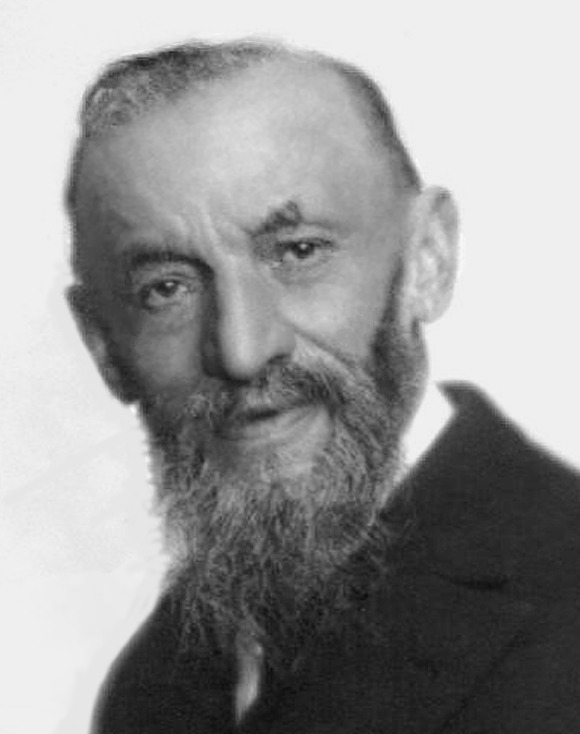
\includegraphics[width=0.5\textwidth]{Peano.jpg}
    \caption{Giuseppe Peano (1858-1932)}
    \label{fig:Peano}
\end{figure}

\begin{aufgabe}{aufgabe:0101}
{Beweisen Sie, dass $2$ eine natürliche Zahl ist. Verwenden Sie dazu lediglich die beiden ersten Peano-Axiome.}
\end{aufgabe}
\noindent
Bereits Giuseppe Peano stellte fest, dass diese ersten beiden Axiome nicht ausreichend sind, um unsere intuitive Vorstellung der natürlichen Zahlen einzufangen. Es könnte sein, dass wir bei dem Vorwärtszählen schliesslich wieder bei $0$ ankommen. Betrachten wir dazu ein Modell der natürlichen Zahlen, welches von $3$ zurück zur $0$ zählt, genauer: $\nu(0)$ ist $1$, $\nu(1)$ ist 2, $\nu(2)$ ist $3$, aber $\nu(3)$ ist wieder $0$ (und gemäss der Definition von $4$ auch gleich der $4$). So erfüllt also auch die Menge $\lrc{0,1,2,3}$ die ersten zwei Peano-Axiome und könnte als Menge der natürlichen Zahlen angesehen werden.
\begin{aufgabe}{aufgabe:0102}
{Welches ist die kleinste Menge, welche die ersten zwei Peano-Axiome erfüllt?}
\end{aufgabe}
\noindent
Die \cref{axiom:a1,axiom:a2} erlauben also auch Mengen, welche wir sicherlich nicht als Modelle der natürlichen Zahlen anschauen möchten. Wir müssen die erlaubten Nachfolger der Elemente der Mengen weiter einschränken. Auf jeden Fall stellen wir fest, dass die $0$ nicht Nachfolger einer natürlichen Zahl sein soll und fordern deshalb:
\axiom{axiom:a3}
{Die $0$ selbst ist nicht der Nachfolger einer natürlichen Zahl.} %Es gilt also $\nu(n)\neq 0$ für jede natürliche Zahl $n$.}

\bemerkung{bemerkung:Nunit}{
Wir bezeichnen mit $\Nunit$ die Menge der natürlichen Zahlen ohne die $0$. Für jede natürliche Zahl $n$ soll der Nachfolger $\nu(n)$ von $n$ wieder eine natürliche Zahl sein. Da gemäss \cref{axiom:a3} die $0$ nicht Nachfolger einer natürlichen Zahl ist, können wir uns $\nu$ als Funktion
\begin{align*}
    \nu: \N&\to\Nunit, \\
    n &\mapsto \nu(n)
\end{align*}
denken. Diese erhält eine natürliche Zahl $n$ als Eingabe und liefert die natürliche Zahl $\nu(n)$, welche nicht die $0$ ist, als Ausgabe.
}
\begin{aufgabe}{aufgabe:0103}
{Beweisen Sie, dass $0\neq 3$ gilt. Verwenden Sie lediglich die ersten drei Peano-Axiome.}
\end{aufgabe}
\noindent
Betrachten Sie ein Zahlensystem, welches $0$ enthält und für das gilt: $\nu(0)$ ist $1$, $\nu(1)$ ist 2, $\nu(2)$ ist $3$, aber $\nu(3)$ bleibt $3$ (also $4=3$, $5=3$, $6=3$ und so weiter). Es ist auch ein Zahlensystem vorstellbar, welches von $3$ zurück zu $1$ geht, also $\nu(3)=1, \nu(1)=2, \nu(2)=3, \nu(3)=1$ und so weiter. Die beiden Beispiele erfüllen alle drei ersten Peano-Axiome. Das Problem ist, dass die ersten drei Peano-Axiome erlauben, dass verschiedene natürliche Zahlen gleiche Nachfolger haben können. Diese Möglichkeit wollen wir also ausschliessen. Dazu fügen wir das vierte Peano-Axiom hinzu:
\axiom{axiom:a4}
{Unterschiedliche natürliche Zahlen haben unterschiedliche Nachfolger. Sind also $n,m$ natürliche Zahlen und $n\neq m$, dann gilt $\nu(n)\neq\nu(m)$. Die Kontraposition dieser Aussage lautet: Gilt $\nu(n)=\nu(m)$, dann folgt $n=m$.}
\begin{aufgabe}{aufgabe:0104}
{Verwenden Sie die ersten vier Peano-Axiome, um zu beweisen, dass $1\neq 4$ gilt.}
\end{aufgabe}
\noindent
Wir wollen $\N$ als die Menge verstehen, welche die $0$ enthält und alle Objekte, welche aus $0$ durch Inkrementieren erhalten werden kann. Diese Intuition wird schliesslich auf geniale Weise durch das fünfte Peano-Axiom formalisiert. Dieses letzte Peano-Axiom formuliert auf mathematisch präzise Weise, was mit \enquote{aus $0$ durch Inkrementieren erhalten werden kann}, gemeint ist:
\axiom{axiom:a5}
{Enthält eine Teilmenge $N\subseteq\N$ das Element $0$ und mit jedem $n\in N$ auch den Nachfolger $\nu(n)$ von $n$, so gilt $N=\N$.}

\subsection{Kompakte Formulierung der Peano-Axiome}\label{subsec:kompakt}
Unser Wissen über Funktionen und ihre Eigenschaften erlaubt uns, die fünf \cref{axiom:a1,axiom:a2,axiom:a3,axiom:a4,axiom:a5}, kompakt und sehr präzise in der folgenden Definition zusammenzufassen:
\begin{definition}[Formale Definition der natürlichen Zahlen]{definition:N}
Die \textbf{natürlichen Zahlen} sind eine Menge $\N$, in der ein Element $0\in\N$ ausgezeichnet ist und für die es eine Funktion $\nu:\N\to\Nunit$ (siehe \cref{bemerkung:Nunit}) mit den folgenden zwei Eigenschaften gibt:
\begin{itemize}
  \item[(N$_0$)] Die Funktion $\nu$ ist injektiv.
  \item[(N$_1$)] Enthält eine Teilmenge $N\subseteq\N$ das Element $0$ und mit jedem $n\in N$ auch den Nachfolger $\nu(n)$ von $n$, so gilt $N=\N$.
\end{itemize}
\end{definition}
Dabei bezeichnet $\Nunit:=\N\setminus{\lrc{0}}$ die Menge der natürlichen Zahlen ohne die $0$. Das Element $\nu(n)$ heisst Nachfolger von $n$ und $\nu$ heisst Nachfolgerfunktion. Die Eigenschaft (N$_1$) ist identisch zum \cref{axiom:a5} und wird auch \tib{Induktionsaxiom}\index{Induktionsaxiom} genannt.
\begin{aufgabe}{aufgabe:0105}
Weisen Sie nach, dass \cref{definition:N} zu den Peano-Axiomen äquivalent ist.
\end{aufgabe}

\begin{aufgabe}{aufgabe:0107}
(*!) Erfüllt auch die Menge $\lrc{0,2,4,6,\ldots}$  der geraden natürlichen Zahlen die Peano-Axiome?
\end{aufgabe}

\begin{aufgabe}{aufgabe:0106}
(*!) Begründen Sie, dass die Nachfolgerfunktion $\nu:\N\to\Nunit$ bijektiv ist.

\noindent
Tipp: Verwenden Sie die beiden Eigenschaften N$_0$ und N$_1$ in \cref{definition:N}.
\end{aufgabe}

\bemerkungen{-}{}
{Aus den grundlegenden Axiomen der Mengenlehre folgt, dass es in der Tat Systeme $(\N,0,\nu)$ gibt, welche die Peano-Axiome erfüllen. Diese Modelle der natürlichen Zahlen sind bis auf die Benennung der Elemente gleichwertig und ergeben dieselbe Mathematik. Beispielsweise könnte man anstelle der arabischen Zahlenschrift auch die römische Zahlenschrift verwenden. Die konkrete Wahl der Symbole ist mathematisch nicht von Bedeutung. Deshalb ist es sinnvoll, von \textit{den} natürlichen Zahlen zu sprechen.}
{Die aus der Schule bekannten Rechenregeln in den natürlichen Zahlen (zum Beispiel das Distributivgesetz) lassen sich allein durch logische Folgerungen aus den Peano-Axiomen beweisen. Diese Beweise werden zum Beispiel in dem Buch \cite{Landau} geführt, welches im Jahr 1930 erschien. Im Vorwort dieses Buchs schreibt der Autor \textit{Edmund Landau} unter anderem:
\begin{itemize}
    \item \enquote{Ich setze nur logisches Denken und die deutsche Sprache als bekannt voraus; nichts aus der Schulmathematik oder gar der höheren Mathematik.}
    \item \enquote{Bitte vergiß alles, was Du auf der Schule gelernt hast; denn Du hast es nicht gelernt.}
\end{itemize}
Wir werden diese (recht umfangreichen) Beweise hier nicht führen. Besonders interessierten Lesenden empfehlen wir in diesem Zusammenhang die entsprechenden Teile in den Büchern \cite{Landau,TerenceTao,AmannEscher1} zu studieren.}

\begin{figure}[H]
    \centering
    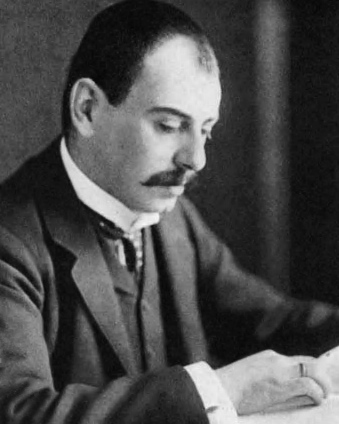
\includegraphics[width=0.4\textwidth]{Landau.jpg}
    \caption{Edmund Landau (1877-1938)}
    \label{fig:Landau}
\end{figure}





\begin{antwort}{aufgabe:0101}
Gemäss \cref{axiom:a1} ist $0$ eine natürliche Zahl. Gemäss \cref{axiom:a2} ist $1=\nu(0)$ eine natürliche Zahl. Schliesslich ist $2=\nu(1)$ wiederum gemäss \cref{axiom:a2} eine natürliche Zahl.
\end{antwort}



\begin{antwort}{aufgabe:0102}
Bereits die Menge $\lrc{0}$ erfüllt die ersten beiden Peano-Axiome. Sie enthält offensichtlich die $0$ und mit $\nu(0):=0$ auch den Nachfolger von jedem $n\in\lrc{0}$ (es gibt nur das eine $n\in\lrc{0}$ und das ist die $0$).
\end{antwort}



\begin{antwort}{aufgabe:0103}
In \cref{aufgabe:0101} haben wir gezeigt, wie aus den ersten zwei Peano-Axiomen folgt, dass $2$ eine natürliche Zahl ist. Definitionsgemäss ist $3=\nu(2)$. Somit ist $3$ der Nachfolger einer natürlichen Zahl und deshalb muss $3$ gemäss dem dritten Peano-Axiom von $0$ verschieden sein, also $0\neq 3$.
\end{antwort}



\begin{antwort}{aufgabe:0104}
Wir beweisen die Aussage durch Widerspruch und nehmen also an, dass $1=4$. Gleichzeitig gilt aber $1=\nu(0)$ und $4=\nu(3)$ und somit $\nu(0)=\nu(3)$. Wegen des vierten Peano-Axioms folgt also $0=3$. Doch in \cref{aufgabe:0103} haben wir gezeigt, dass $0\neq 3$ gilt. Wir haben also einen Widerspruch gefunden und somit muss $1\neq 4$ gelten.
\end{antwort}



\begin{antwort}{aufgabe:0105}
Wir zeigen zuerst, dass \cref{definition:N} alle fünf Peano-Axiome \enquote{abdeckt}.
\begin{itemize}
    \item[\cref{axiom:a1}:] Dieses Axiom ist erfüllt, da in der Definition gefordert wird, dass ein Element $0$ in $\N$ ausgezeichnet ist.
    \item[\cref{axiom:a2}:] Dieses Axiom ergibt sich dadurch, dass $\nu:\N\to\Nunit$ eine Funktion von den natürlichen Zahlen in eine Teilmenge der natürlichen Zahlen ist. Doch die Elemente einer Teilmenge der natürlichen Zahlen sind offensichtlich ebenfalls natürliche Zahlen.
    \item[\cref{axiom:a3}:] Wegen $\nu:\N\to\Nunit$ liegt die $0$ nicht im Bild der Funktion $\nu$. Somit ist also die $0$ nicht Nachfolger einer natürlichen Zahl und damit ist auch dieses Axiom erfüllt.
    \item[\cref{axiom:a4}:] Dieses Axiom sagt genau, dass die Funktion $\nu$ injektiv ist und entspricht somit exakt der Eigenschaft (N$_0$).
    \item[\cref{axiom:a5}:] Dieses Axiom entspricht exakt der Eigenschaft (N$_1$).
\end{itemize}
Da \cref{definition:N} keine zusätzlichen Forderungen stellt, ist diese Definition tatsächlich äquivalent zu den Peano-Axiomen.
\end{antwort}



\begin{antwort}{aufgabe:0107}
Die Frage der Aufgabenstellung geht an der eigentlichen Aussage der Peano-Axiome vorbei und ist im Grunde bedeutungslos. Die Peano-Axiome verlangen nicht, dass die natürlichen Zahlen genau die Form
\begin{align*}
    \lrc{0,1,2,3,4,\ldots}
\end{align*}
haben. Die konkreten Schriftsymbole, mit denen die natürlichen Zahlen bezeichnet werden, werden von den Peano-Axiomen nicht vorgeschrieben. In der üblichen westlichen Schreibweise wird der Nachfolger der $0$ mit dem Symbol $1$ bezeichnet, der Nachfolger von $1$ mit $2$ und so weiter. Anstelle von der Konvention
\begin{align*}
    1:=\nu(0), 2:=\nu(1)=\nu(\nu(0)), 3:=\nu(2)=\nu(\nu(\nu(0))), \ldots
\end{align*}
könnten wir den Nachfolger der $0$ auch mit $2$ bezeichnen und den Nachfolger der $2$ mit $4$ und so weiter. Offensichtlich ist auch das exakte Symbol der Null bedeutungslos. Anstelle von dem Symbol $0$ könnten wir auch das Symbol \twemoji{city_sunset} für dieses ausgezeichnete Element verwenden. Es ist nicht einfach, sich auf diese abstrakte Ebene zu begeben. Sie müssen sich von den konkret verwendeten Schriftsymbolen lösen und sich stattdessen auf die Bedeutung der verwendeten Symbole fokussieren.
\end{antwort}

\begin{antwort}{aufgabe:0106}
Wie können wir beweisen, dass $\nu$ bijektiv ist? Wir dürfen für den Nachweis lediglich bereits bekannte Tatsachen sowie die Peano-Axiome in \cref{definition:N} verwenden. Sicherlich können wir zunächst einmal feststellen, dass die Funktion $\nu$ wegen der Eigenschaft N$_0$ als injektiv vorausgesetzt ist. Damit ist $\nu$ also injektiv. Für den Nachweis der Bijektivität von $\nu$ müssen wir nur noch seine Surjektivität zeigen.

Möchte man eine Eigenschaft nachweisen, ist es zunächst einmal sinnvoll, aufzuschreiben, was diese Eigenschaft genau bedeutet. Definitionsgemäss ist $\nu:\N\to\Nunit$ genau dann surjektiv, wenn das Bild $\text{im}\lr{\nu}$ der Zielmenge $\Nunit$ entspricht, falls also
\begin{align*}
    \textcolor{DarkGreen}{\text{im}\lr{\nu} = \Nunit}
\end{align*}
gilt. Nun haben wir Eigenschaft N$_0$ in \cref{definition:N} bereits ausgenutzt. Es ist daher naheliegend, Eigenschaft N$_1$ zu betrachten. Da N$_1$ eine Aussage über $\N$ und nicht etwa über $\Nunit$ macht, tun wir uns selbst einen Gefallen, wenn wir anstelle von $\Nunit$ die um das Element $0$ erweiterte \enquote{Hilfsmenge}
\begin{align*}
    N := \text{im}\lr{\nu} \cup \lrc{0}
\end{align*}
betrachten. Wir zeigen nun, dass diese Hilfsmenge $N$ eine Teilmenge von $\N$ ist, welche die Bedingungen in N$_1$ erfüllt. Offensichtlich gelten $N\subseteq \N$ und $0\in N$. Für $n\in N$ gilt $\nu(n)\in\text{im}\lr{\nu}\subseteq N$. Somit liegt für $n\in N$ auch der Nachfolger $\nu(n)$ in der Menge $N$ und damit folgt aus N$_1$, dass $N = \N$ gilt. Wir haben also die Gleichheit
\begin{align*}
    \text{im}\lr{\nu} \cup \lrc{0} = \N
\end{align*}
gezeigt und folgern daraus
\begin{align*}
    \textcolor{DarkGreen}{\text{im}\lr{\nu} = \Nunit}.
\end{align*}
\end{antwort}

\clearpage
\shipoutAnswer